%%%%%%%%%%%%%%%%%%%%%%%%%%%%%%%%%%%%%%%%%%%%%%%%
%% Intro to LaTeX and Template for Homework Assignments
%% Quantitative Methods in Political Science
%% University of Mannheim
%% Fall 2017
%%%%%%%%%%%%%%%%%%%%%%%%%%%%%%%%%%%%%%%%%%%%%%%%

% created by Marcel Neunhoeffer & Sebastian Sternberg


% This template and tutorial will help you to write up your homework. It will also help you to use Latex for other assignments than this course's homework.

%%%%%%%%%%%%%%%%%%%%%%%%%%%%%%%%%%%%%%%%%%%%%%%%
% Before we get started
%%%%%%%%%%%%%%%%%%%%%%%%%%%%%%%%%%%%%%%%%%%%%%%%

% Make an account on overleaf.com and get started. No need to install anything.

%%%%%%%%%%%%%%%%%%%%%%%%%%%%%%%%%%%%%%%%%%%%%%%%
% Or if you want it the nerdy way...
% INSTALL LATEX: Before we can get started you need to install LaTeX on your computer.
				% Windows: http://miktex.org/download
				% Mac:         http://www.tug.org/mactex/mactex-download.html	
				% There a many more different LaTeX editors out there for both operating systems. I use TeXworks because it looks the same on Windows and Mac.
				

% SAVE THE FILE: The first thing you need to do is to save your LaTeX file in a directory as a .tex file. You will not be able to do anything else unless your file is saved. I suggest to save the .tex file in the same folder with your .R script and where you will save your plots from R to. Let's call this file template_homework1.tex and save it in your Week 1 folder.


% COMPILE THE FILE: After setting up your file, using your LaTeX editor (texmaker, texshop), you can compile your document using PDFLaTeX.
	% Compiling your file tells LaTeX to take the code you have written and create a pdf file
	% After compiling your file, in your directory will appear four new files, including a .pdf file. This is your output document.
	% It is good to compile your file regularly so that you can see how your code is translating into your document.
	
	
% ERRORS: If you get an error message, something is wrong in your code. Fix errors before they pile up!
	% As with error messages in R, google the exact error message if you have a question!
%%%%%%%%%%%%%%%%%%%%%%%%%%%%%%%%%%%%%%%%%%%%%%%%


% Now again for everyone...

% COMMANDS: 
	% To do anything in LaTeX, you must use commands
	% Commands tell LaTeX when to start your document, how you want your document to look, and how to format your document
	% Commands ALWAYS begin with a backslash \

% Everything following the % sign is a comment and will not be used by Latex to compile your document.
% This is very similar to # comments in R.

% Every .tex file usually consists of four parts.
% 1. Document Class
% 2. Packages
% 3. Header
% 4. Your Document

%%%%%%%%%%%%%%%%%%%%%%%%%%%%%%%%%%%%%%%%%%%%%%%%
% 1. Document Class
%%%%%%%%%%%%%%%%%%%%%%%%%%%%%%%%%%%%%%%%%%%%%%%%
 
 % The first command you will always have will declare your document class. This tells LaTeX what type of document you are creating (article, presentation, poster, etc). 
% \documentclass is the command
% in {} you specify the type of document
% in [] you define additional parameters
 
\documentclass[a4paper,11pt]{article} % This defines the style of your paper

% We usually use the article type. The additional parameters are the format of the paper you want to print it on and the standard font size. For us this is a4paper and 12pt.

%%%%%%%%%%%%%%%%%%%%%%%%%%%%%%%%%%%%%%%%%%%%%%%%
% 2. Packages
%%%%%%%%%%%%%%%%%%%%%%%%%%%%%%%%%%%%%%%%%%%%%%%%

% Packages are libraries of commands that LaTeX can call when compiling the document. With the specialized commands you can customize the formatting of your document.
% If the packages we call are not installed yet, TeXworks will ask you to install the necessary packages while compiling.

% First, we usually want to set the margins of our document. For this we use the package geometry. We call the package with the \usepackage command. The package goes in the {}, the parameters again go into the [].
\usepackage[top = 2cm, bottom = 2cm, left = 2 cm, right = 2cm]{geometry} 

% Unfortunately, LaTeX has a hard time interpreting German Umlaute. The following two lines and packages should help. If it doesn't work for you please let me know.
\usepackage[T1]{fontenc}
\usepackage[utf8]{inputenc}

% The following two packages - multirow and booktabs - are needed to create nice looking tables.
\usepackage{multirow} % Multirow is for tables with multiple rows within one cell.
\usepackage{booktabs} % For even nicer tables.

% As we usually want to include some plots (.pdf files) we need a package for that.
\usepackage{graphicx} 

% The default setting of LaTeX is to indent new paragraphs. This is useful for articles. But not really nice for homework problem sets. The following command sets the indent to 0.
\usepackage{setspace}
\setlength{\parindent}{0in}
\setlength{\parskip}{0.25em}
% Package to place figures where you want them.
\usepackage{float}
\usepackage{minted}
% The fancyhdr package let's us create nice headers.
\usepackage{fancyhdr}

\usepackage{amsmath,amssymb}
\usepackage{xcolor}
\usepackage{hyperref}
\hypersetup{
    colorlinks=true,
    linkcolor=blue,
    filecolor=magenta,      
    urlcolor=cyan,
}
\usepackage{soul} % for highlighting
\usepackage{graphicx} % graphics package
\usepackage{caption}
\usepackage{subcaption} % subplot package
\graphicspath{{images/}} % declare the path where graphic files are
\DeclareGraphicsExtensions{.pdf,.jpg,.png} % grafic files extensions
\usepackage{epstopdf} % package to include eps. files
\usepackage{float}
\usepackage{booktabs}
\usepackage{array}
\usepackage[linesnumbered, ruled]{algorithm2e}
\usepackage{ulem}
\usepackage{mdframed}
\soulregister\ref7
\soulregister\cite7
\soulregister\url7
\newcommand{\highlight}[1]{\colorbox{yellow}{$\displaystyle#1$}}

%%%%%%%%%%%%%%%%%%%%%%%%%%%%%%%%%%%%%%%%%%%%%%%%
% 3. Header (and Footer)
%%%%%%%%%%%%%%%%%%%%%%%%%%%%%%%%%%%%%%%%%%%%%%%%

% To make our document nice we want a header and number the pages in the footer.

\pagestyle{fancy} % With this command we can customize the header style.

\fancyhf{} % This makes sure we do not have other information in our header or footer.

\lhead{\footnotesize \assType\ \exeNum}% \lhead puts text in the top left corner. \footnotesize sets our font to a smaller size.

%\rhead works just like \lhead (you can also use \chead)
\rhead{\footnotesize \studentName} %<---- Fill in your lastnames.

% Similar commands work for the footer (\lfoot, \cfoot and \rfoot).
% We want to put our page number in the center.
\cfoot{\footnotesize \thepage} 

%----------------------------------------------------------------------------------------
%	WORK EXPERIENCE FORMATTING
%----------------------------------------------------------------------------------------
% set line spacing
\newcommand{\lineSpace}{1.1}

% syntax: \newenvironment{name}{begin command}{endcommand}
\newcounter{rSection}
\newcounter{rSubsection}[rSection]
% update the subsection counter to sec_counter.subsec_counter
% so it works correctly in cross references
\renewcommand{\therSubsection}{\therSection.\arabic{rSubsection}} 

\newenvironment{rSection}[1]{ % 1 input argument - section name
\refstepcounter{rSection}
\begin{spacing}{\lineSpace}
  {\bf \large \therSection~#1 \hfill}  % Section title DO NOT delete the following blank line
	\vspace{0.25em}

}{
\vspace{1em}
\end{spacing}
}

\newenvironment{rSubsection}[1]{ % 1 input argument - section name
  \refstepcounter{rSubsection}
  \begin{spacing}{\lineSpace}
	{\bf\therSubsection~#1}

  }{
\end{spacing}
\vspace{0.5em}
}


\newenvironment{rlisting}{
  \vspace{-0.5em}
  \begin{itemize}
	\itemsep -0.25em \vspace{-0.5em}
}{
	\vspace{-0.5em}
\end{itemize}
\vspace{-0.5em}
}

\newenvironment{renum}{
	\vspace{-0.5em}
  \begin{enumerate}
	\itemsep -0.25em \vspace{-0.5em}
}{
	\vspace{-0.5em}
\end{enumerate}
\vspace{-0.5em}
}

\definecolor{bg}{rgb}{0.95,0.95,0.95}
\renewcommand\refname{\large References}
%%%%%%%%%%%%%%%%%%%%%%%%%%%%%%%%%%%%%%%%%%%%%%%%
% 4. Your document
%%%%%%%%%%%%%%%%%%%%%%%%%%%%%%%%%%%%%%%%%%%%%%%%

% Now, you need to tell LaTeX where your document starts. We do this with the \begin{document} command.
% Like brackets every \begin{} command needs a corresponding \end{} command. We come back to this later.

%%%%%%%%%%%%%%%%%%%%%%%%%%%%%%%%%%%%%%%%%%%%%%%%%%%%%%
\newcommand{\exeNum}{}
\newcommand{\assType}{Normalizing Flows for Implicit Bayesian Neural Networks}
\newcommand{\courseName}{Project Summary}
\newcommand{\semester}{Summer 2021}
\newcommand{\studentName}{Weijiang Xiong}
\newcommand{\studentNumber}{875581}
%%%%%%%%%%%%%%%%%%%%%%%%%%%%%%%%%%%%%%%%%%%%%%%%%%%%%%
\begin{document}
\linespread{\lineSpace} % line spacing

%%%%%%%%%%%%%%%%%%%%%%%%%%%%%%%%%%%%%%%%%%%%%%%%
%%%%%%%%%%%%%%%%%%%%%%%%%%%%%%%%%%%%%%%%%%%%%%%%

%%%%%%%%%%%%%%%%%%%%%%%%%%%%%%%%%%%%%%%%%%%%%%%%
% Title section of the document
%%%%%%%%%%%%%%%%%%%%%%%%%%%%%%%%%%%%%%%%%%%%%%%%

% For the title section we want to reproduce the title section of the Problem Set and add your names.

\thispagestyle{empty} % This command disables the header on the first page. 

\begin{tabular}{p{16.5cm}} % This is a simple tabular environment to align your text nicely 
{\large \bf \courseName \hfill \semester} \\
\hline % \hline produces horizontal lines.
\\
\end{tabular} % Our tabular environment ends here.

% \vspace{0.3cm} % Now we want to add some vertical space in between the line and our title.

\begin{center} % Everything within the center environment is centered.
	{\Large \bf \assType\ \exeNum} % <---- Don't forget to put in the right number

	% {\studentName\ (Student Number \studentNumber)} % <---- Fill in your names here!
	\vspace{1em}

	{Student: \studentName \qquad Supervisor: Markus Heinonen}
\end{center}  
% 

%%%%%%%%%%%%%%%%%%%%%%%%%%%%%%%%%%%%%%%%%%%%%%%%
%%%%%%%%%%%%%%%%%%%%%%%%%%%%%%%%%%%%%%%%%%%%%%%%

% Up until this point you only have to make minor changes for every week (Number of the homework). Your write up essentially starts here.
\begin{rSection}{Introduction and Motivation}
\begin{rSubsection}{Types of Uncertainties in Deep Learning}
Deep learning methods have led to significant advances in research on Artificial Intelligence. 
Typically, we will create a model $\mathcal{M}$ to capture the patterns in a given dataset $\mathcal{D}$.
More specifically, for supervised learning tasks, the dataset usually consists of pairs of inputs and labels $(\mathbf{X}, \mathbf{y})$.
Thus, the problem can be described as: choosing an optimal set of parameters $\mathbf{w}$ for the model $\mathcal{M}$, so the model prediction $\mathcal{M}_{\mathbf{w}}(\mathbf{X})$ is closest to the label $\mathbf{y}$ under a distance measurement (loss function) $\mathcal{L}$.

While the optimizing problem of parameter $\mathbf{w}$ can be tackled by error backpropagation and gradient-based approaches, such as ADAM~\cite{kingma2014adam}, there is no guarantee of an optimal parameter set $\mathbf{w}$.
On the contrary, in practice, we will randomly initialize $\mathbf{w}$ and then start an learning algorithm.
And it's often the case that the learning algorithm behaves stably, which means if we run the same training program multiple times, the different obtained models will have comparable training losses after several epochs, and also similar accuracies on test data. 
Those models have different initial parameters, and will end up having different weights after learning process.

A question that rises is how to make use of those models.
In practice, we often pick the one with highest test accuracy, even if those models have almost equal performance.
However, with the accuracy on the limited testing data, we are not sure whether the picked model is the \textit{truly best} model that correctly models the true data-generating process. 
Therefore, in Bayesian Deep Learning, we model this uncertainty with a probability distribution over the weights $p(\mathbf{w} | \mathcal{D})$, which is known as \textit{epistemic uncertainty} or simply \textit{weight uncertainty}. 
And this kind of neural network is known as Bayesian Neural Network (BNN), which marginalize over the weight posterior to provide predictive distributions~\cite{wilson2020bayesian}:
\begin{equation}
	p(\mathbf{y} \mid \mathbf{X}, \mathcal{D})
	=
	\int p(\mathbf{y} \mid \mathbf{X}, \mathbf{w}) p(\mathbf{w} \mid \mathcal{D}) d \mathbf{w}.
\end{equation}
As we obtain more data, the results on the dataset will be more reliable, and thus weight uncertainty could be explained away with enough data~\cite{kendall2017uncertainties}.

On the other hand, real-world data are often captured by sensors, for example, images are taken by cameras and audio waves are recorded by microphones. 
As a result, sensor noise and motion noise will lead to uncertainties in recorded data. 
Figure \ref{fig: intro example} (a) shows an example of motion blur, where the images of some moving people become unclear.
This kind of uncertainty is known as \textit{aleatoric uncertainty} or simply \textit{input uncertainty}.
Unfortunately, aleatoric uncertainty is inherent in data, and can not be explained away even if we obtain more data \cite{kendall2017uncertainties}.

\begin{figure}[H]
\centering
\begin{subfigure}[t]{0.26\textwidth}
	\centering	
	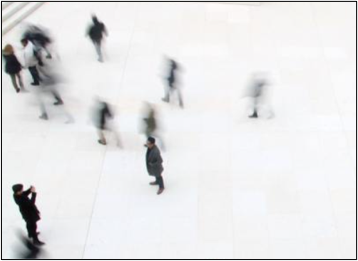
\includegraphics[width=\textwidth]{figs/s1_motion_blur.png}
	\caption{Motion Blur}
\end{subfigure}
\begin{subfigure}[t]{0.65\textwidth}
	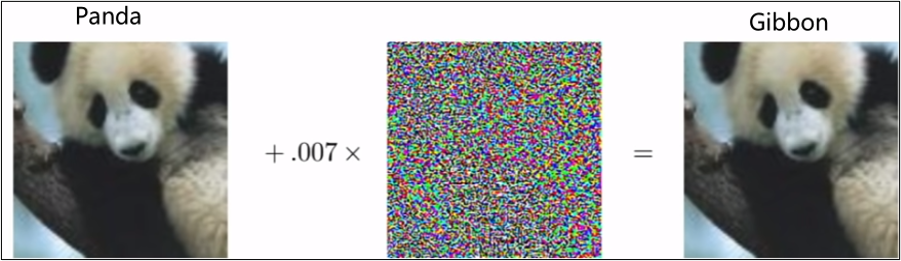
\includegraphics[width=\textwidth]{figs/s1_adversarial_attack.png}
	\caption{Adversarial Attack}
\end{subfigure}
\caption{}
\label{fig: intro example}
\end{figure}

\end{rSubsection}

\begin{rSubsection}{Motivation for Modelling Uncertainties}
\label{subsec: motivation}
In this project, we study the uncertainty modelling problem in the context of image classification, a basic task in computer vision. 
The motivation comes from two problems in deep neural networks. 

First, conventional DNNs are considered to be deterministic.
Because they only learn a single set of parameters, and thus providing a point estimation.
However, from the discussions above, we see that uncertainty exists in both the network weight and input data. 
Moreover, in applications that involves decision making (such as autonomous driving), we would like to consider all probable results and make sure the decision won't violate any rules or hurt anybody in all these conditions.
Thus, uncertainties must be seriously taken into account, and a point estimation won't be sufficient.

Second, DNNs are usually overconfident about its results~\cite{guo2017calibration}, even if the results are wrong. 
Figure~\ref{fig: intro example}~(b) shows an adversarial example~\cite{goodfellow2017ganlecture}, where we mix a carefully-chosen noise image to the image of a panda.
As a result, the network classifies the mixed image as a gibbon with very high confidence. 
This error-prone overconfidence makes the output of DNNs even less reliable.
Therefore, we would like to learn a model that is \textit{well-calibrated}, which means it's confidence should match the actual accuracy. 
Then the distribution of confidence will reflect the uncertainties of the prediction.

In short, an ideal model should learn the uncertainties its task and provide trustworthy confidence.

\end{rSubsection}

\begin{rSubsection}{Project Idea}

In theory, we may consider both epistemic uncertainty and aleatoric uncertainty, but previous research has shown that for computer vision tasks, it's more efficient to model input uncertainty rather than weight uncertainty~\cite{kendall2017uncertainties,trinh2020ibnn}.
For a deep neural network with millions of parameters, placing a distribution on weights is computationally expensive, but the input space makes a more suitable option.
Because the size of an image or a feature map is usually much smaller than the network itself.

Trinh et al.~\cite{trinh2020ibnn} proposed an implicit Bayesian Neural Network (iBNN) that learns a Gaussian distribution for the input noise in each network layer. 
Compared to conventional neural networks, iBNN achieves higher classification accuracy and is also better calibrated.
Although the variance of Gaussian distribution provides a reasonable estimation for uncertainties, real-world image data have various contents and the true input uncertainty could have more complicated distributions.
Therefore, in this project, we will further extend the iBNN with Normalizing Flows~\cite{rezende2015variational} to support more flexible distributions.

\end{rSubsection}

\end{rSection}

\begin{rSection}{Normalizing Flows for Implicit BNN}
\label{sec: nf for ibnn}
\begin{rSubsection}{General Network Structure}
The general structure of iBNN-style network is similar to conventional deep neural network.
As shown in Figure~\ref{fig: network structure}, an iBNN-style network contains a series of deterministic layers and stochastic layers. 
These two kinds of layers have the same interface, i.e., the same format for input and output, but different internal mechanisms.
A deterministic layer refers to the building blocks of conventional neural network, such as convolution layer and linear layer.
Meanwhile, A stochastic layer extends a deterministic layer with a stochastic branch that offers a random vector to augment the original input. 
The workflow can also be expressed with the following equations.

\begin{equation}
\begin{aligned}
\mathbf{f}_{l}(\mathbf{x}) 
&=layer_{l}\left(\mathbf{z}_{l} \circ \mathbf{f}_{l-1}\right) \quad l \geq 1\\
\mathbf{f}_{0} &=\mathbf{x} \\
\mathbf{z}_{l} & = NF_l(\mathbf{z}_0) \\
\mathbf{z}_0 & \sim q_0(\mathbf{z})
\end{aligned}
\end{equation}

In the forward pass of a stochastic layer (indexed by $l$), we first sample a (set of) stochastic vector(s) $\mathbf{z}_0$ from the base distribution $q_0(\mathbf{z})$ (Base Dist.).
Then, the base samples $\mathbf{z}_0$ will go through a stack of Normalizing Flows (NF), which apply a series of invertible transforms to the input samples and output transformed samples $\mathbf{z}_l$.
After that, the transformed samples will augment the output of the previous layer, i.e. $\mathbf{f}_{l-1}$, through element-wise multiplication.
Finally, we put the augmented input $\mathbf{z}_l \circ \mathbf{f}_{l-1}$ into the deterministic component (Det. Compo) of that stochastic layer, which is literally a deterministic layer. 

To represent the flow based distribution, we will need a number of samples.
Therefore an input image will be augmented by different transformed samples, and the output will also consists of different samples, from which we can learn the output uncertainty. 
\begin{figure}[H]
	\centering
	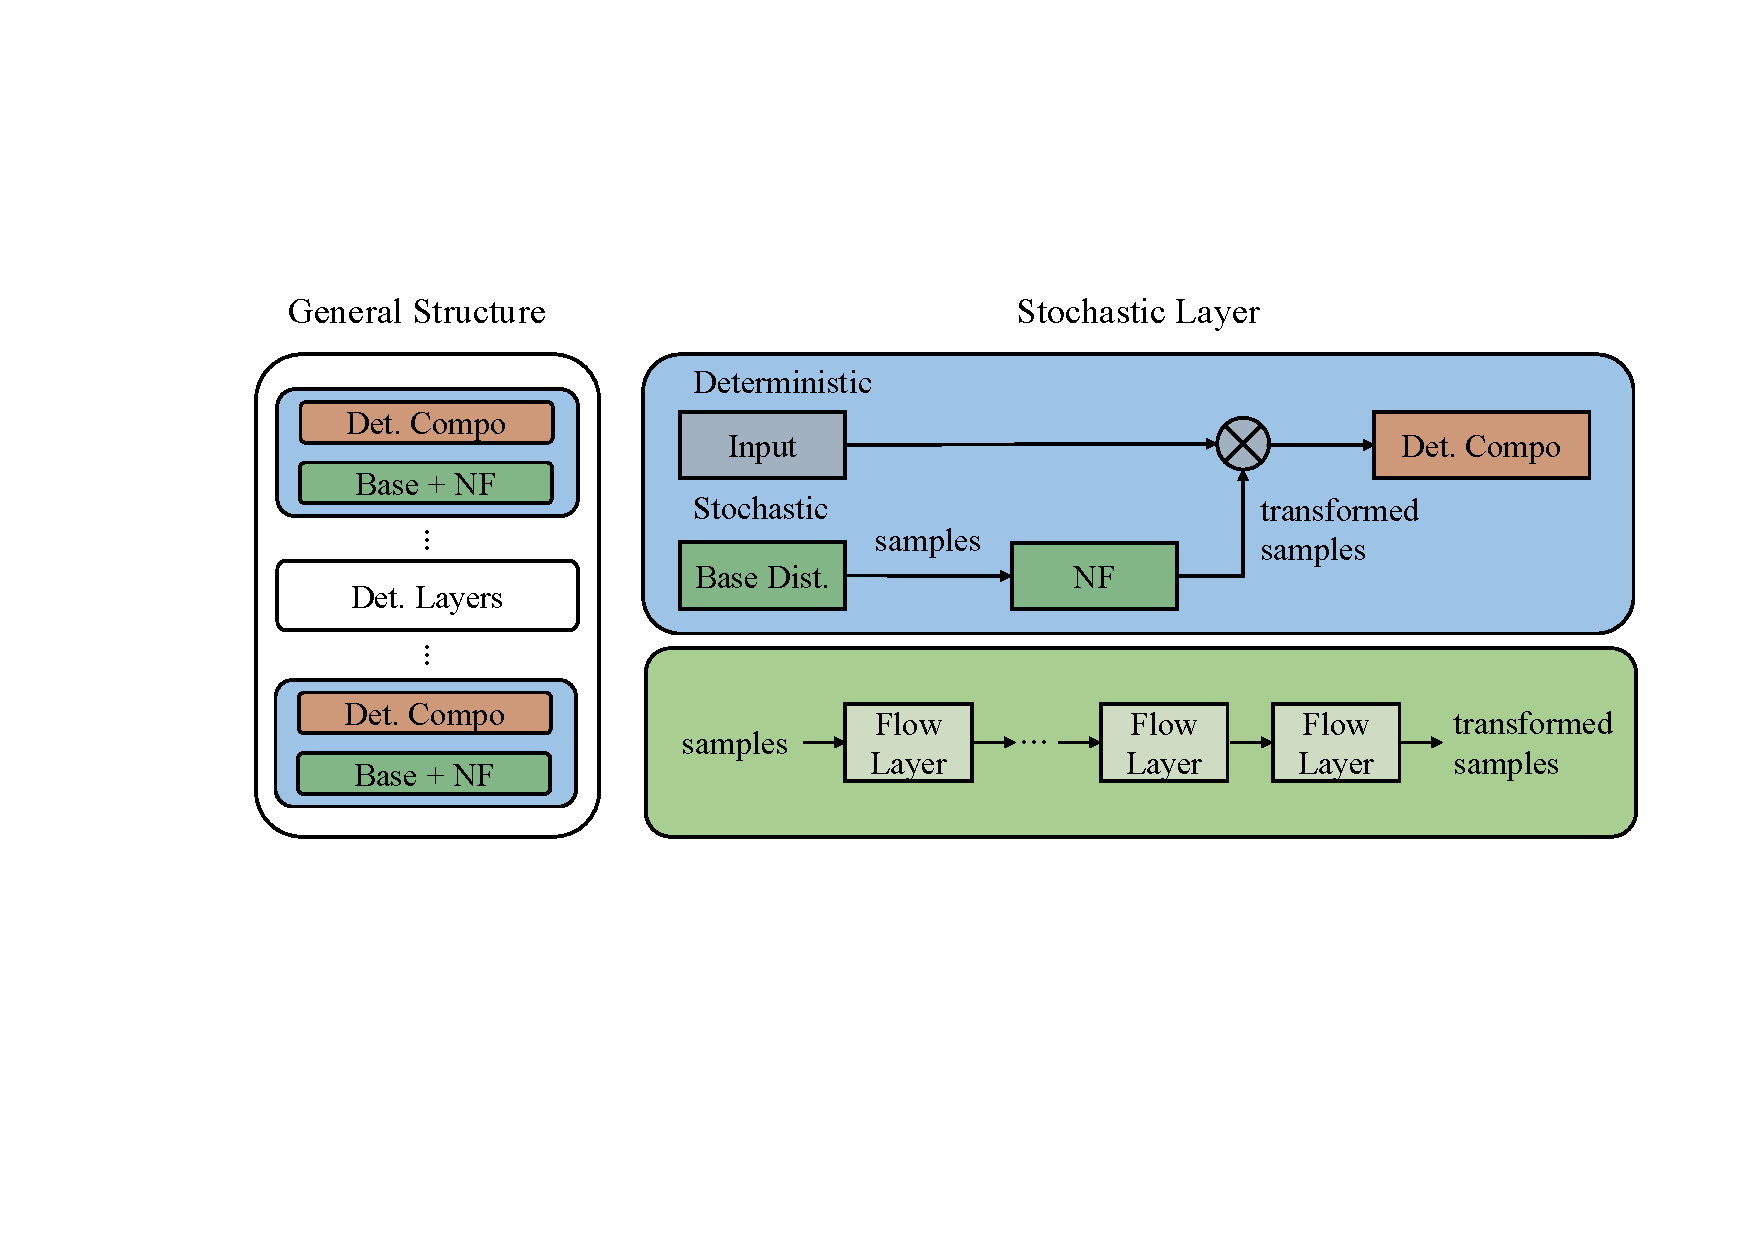
\includegraphics[width=0.95\textwidth]{figs/general structure.pdf}
	\caption{Network Structure}
	\label{fig: network structure}
\end{figure}
\end{rSubsection}

Notably, we assume that each layer has its own stochastic part, which is independent from other layers.
Besides, the deterministic and stochastic part could be trained separately, and we can even migrate the weights for deterministic part from a pre-trained model. 
From this perspective, we can also regard the stochastic part as an extension to the original neural network. 

\begin{rSubsection}{Properties Normalizing Flows}
In probabilistic modeling and inference, we often need to find a balance between expressiveness and tractability.
While simple distributions, such as Gaussian,  have nice analytical properties and is efficient to compute, their expressiveness is also highly limited.
Sometimes even if we just move one step more complicated, the problem instantly lose analytical solution. 
For example, the KL divergence of two Gaussian distributions have closed form solution, but if we change one of them into a mixture of Gaussian, there won't be general solution anymore. 

Normalizing Flows are a series of bijective (invertible) functions, with which we can construct arbitrarily complex distributions from a simple distribution. 
In recent years, Normalizing Flows have been successfully applied to density estimation~\cite{rezende2015variational} and image generation~\cite{kingma2018glow}, where the exact value of parameters are learned from data. 
These research works have shown the expressiveness of NFs, and in this project, we will apply them to image classification task and learn the uncertainties of images and feature vectors. 

Mathematically, a normalizing flow consists of one or several invertible transforms:
\begin{equation}
	\begin{aligned}
		\mathbf{z}_k 
		&= g_{k} ( g_{k-1} (\ldots g_{1}(\mathbf{z}_0)))\\
		&= g_{k} \circ g_{k-1} \circ \ldots \circ g_{1}(\mathbf{z}_0),
	\end{aligned}
\end{equation}
where $g_1, \ldots, g_k$ are invertible functions, $\mathbf{z}_0$ is a continuous random variable with simple distribution (such as Gaussian) and $\mathbf{z}_k$ is the transformed random variable with a complex distribution.
The key benefit is that we can evaluate the log probability density value of $\mathbf{z}_k$ with the following equation:
\begin{equation}
	\label{equ: nf density}
	\begin{aligned}
		\log q(\mathbf{z}_k) 
		&= \log \left[ q_0(\mathbf{z}_0) \prod_{i=1}^k\left|  \det J_{g_i}(\mathbf{z}_{i-1})\right|^{-1} \right] 
		=\log q_0(\mathbf{z}_0) - \sum_{i=1}^k \log \left| \det J_{g_i}(\mathbf{z}_{i-1})\right|.
	\end{aligned}
\end{equation}
While $\log q_0(\mathbf{z}_0)$ is the log probability of the initial random variable (base distribution), the second term accounts for the transformations made by the $k$ layers of flows. 
First, $\mathbf{z}_{i-1}$ means the random variable transformed by previous $i-1$ layers of flow, i.e., $\mathbf{z}_{i-1} = g_{i-1}\circ \ldots \circ g_{1}(\mathbf{z}_0)$.
Then, $J_{g_i}(\mathbf{z}_{i-1})$ computes the Jacobian matrix of the $i$-th layer of flow with respect to its immediate input $\mathbf{z}_{i-1}$.
After that, we compute the determinant ($\det$) of the Jacobian matrix, take its absolute value ($|\cdot|$) and then map to log space ($\log$).  
For a tutorial on normalizing flow, please refer to~\cite{eric2018NFtutorial}, and for detailed proof please have a look at~\cite{papamakarios2019normalizing}.

But here is an simplified example.
Consider a general function $y=f(x)$, where $x$ is a Gaussian random variable.
Then a small interval on the $x$ axis $[x, x+dx]$ is mapped to $[y, y+dy]$.
If we think of the corresponding probability mass on the two intervals like a physical flow (wind), the total probability mass will stay the same, just like the mass stays the same in a physical flow.
Meanwhile, the density and volume could change because of outer environment. 
For wind, that would be different pressure in the atmosphere.
But the product of density and volume, i.e., mass, must not change. 
In in our example, density becomes probability density $p(x)$ and $p(y)$, and volume becomes $|dx|$ and $|dy|$.
Here we take the absolute value because volume is always positive, but $|dx|$ and $|dy|$ could be either positive or negative.
Therefore we have an equation $p(x)|dx| = p(y)|dy|$, which is even simpler in log space:
\begin{equation}
	\log p(y) = \log p(x) - \log |\frac{dy}{dx}|.
\end{equation}
Similarly, if we have another function $z=g(y)$, then 
\begin{equation}
	\log p(z) = \log p(y) - \log |\frac{dz}{dy}|.
\end{equation}
Adding up the two equations we know the log probability density of random variable $z$:
\begin{equation}
	\log p(z) = \log p(x) - (\log |\frac{dz}{dy}| + \log |\frac{dy}{dx}|)
\end{equation}
In fact, we know the source of $z$ can be traced back to $x$, because $z=g(y)=g(f(x))$, but the distribution of $z$ could be much more complicated than $x$ because of the changes induced by $f$ and $g$.
If we generalize into vector case from scalar case, the derivatives $\frac{dz}{dy}$ and $\frac{dy}{dx}$ will also become Jacobian matrices.
Then we will have Equation~\ref{equ: nf density}.
\end{rSubsection}

\begin{rSubsection}{Examples of Flow}
Although Equation~\ref{equ: nf density} provides a straightforward method for density evaluation, the Jacobian determinant $\det J_{g_i}(\mathbf{z}_{i-1})$ in the expression makes it computationally expensive. 
Specifically, a recent research on matrix multiplication has indicated a complexity at $\mathcal{O}(n^{2.37})$~\cite{alman2021refined}.
Therefore, we still need to carefully choose the functions in the flow stack to have feasible determinant computation. 
In this section, we will briefly introduce three kinds of flows with tractable Jacobian determinant: planar flow~\cite{rezende2015variational}, affine coupling flow~\cite{dinh2016density} and $1\times 1$ invertible convolution~\cite{kingma2018glow}.

\textbf{Planar Flow} belongs to the Residual Flow family~\cite{papamakarios2019normalizing}, which means the transformed vector $\mathbf{z}'$ is a sum of the original vector $\mathbf{z}$ and a residual term. 
Equation~\ref{equ: planar flow} shows the transform, Jacobian matrix and the Jacobian determinant of planar flow.
Notably, we need to use the Matrix Determinant Lemma to get the final expression of Jacobian determinant.
\begin{equation}
	\label{equ: planar flow}
	\begin{aligned}
		\mathbf{z}^{\prime}
		&=\mathbf{z}+\mathbf{v} \sigma\left(\mathbf{w}^{\top} \mathbf{z}+b\right) \\
		J_{g}(\mathbf{z})
		&=\mathbf{I}+\sigma^{\prime}\left(\mathbf{w}^{\top} \mathbf{z}+b\right) \mathbf{v} \mathbf{w}^{\top} \\
		\operatorname{det} J_{g}(\mathbf{z})&=1+\sigma^{\prime}\left(\mathbf{w}^{\top} \mathbf{z}+b\right) \mathbf{w}^{\top} \mathbf{v}
	\end{aligned}
\end{equation}

\textbf{Affine Coupling Flow} splits the input vector into two groups, keep one group unchanged, and apply element-wise transform to the other group.
\begin{equation}
	\begin{aligned}
		\mathbf{z}'_{1: d} &=\mathbf{z}_{1: d} \\
		\mathbf{z}'_{d+1: D} &=\mathbf{z}_{d+1: D} \odot \exp \left(s\left(\mathbf{z}_{1: d}\right)\right)+t\left(\mathbf{z}_{1: d}\right)
	\end{aligned}
\end{equation}
Here, the first $d$ elements $\mathbf{z}_{1: d}$ belongs to a group, and the rest $\mathbf{z}_{d+1: D}$ belongs to another.
Meanwhile, $s(\cdot)$ and $t(\cdot)$ can be any functions. 
As a result, the Jacobian matrix will be triangular (Equation~\ref{equ: affine coupling}), and thus the determinant will be the product of diagonal elements. 
Usually we need the log of determinant, which turns out to be the sum of elements in $s(\mathbf{z}_{1: d})$.
\begin{equation}
	\label{equ: affine coupling}
	\begin{aligned}
	J_g(\mathbf{z})^\top
	&=
	\left[\begin{array}{cc}
	\mathbf{I}_{d} &  0\\
	\frac{\partial \mathbf{z}'_{d+1: D}}{\partial \mathbf{z}_{1: d}} & \operatorname{diag}\left(\exp \left[s\left(\mathbf{z}_{1: d}\right)\right]\right)
	\end{array}\right] \\
	\log \det J_g(\mathbf{z}) &= \operatorname{sum}(s(\mathbf{z}_{1: d}))
	\end{aligned}
\end{equation}


\textbf{$1 \times 1$ Invertible Convolution} is specially adapted for image data, and apply a shared weight matrix $\mathbf{W}$ across the height and width dimensions.
If we have an input image or feature map with size $(C, H, W)$, the size of weight matrix will be $C \times C$.
Then, for each length-$C$ feature vector $\mathbf{z}_{i,j}$ across the height and width dimensions, we have the following equations:
\begin{equation}
	\begin{aligned}
	\mathbf{z}'_{i,j} &= \mathbf{W}\mathbf{z}_{i,j}\\
	J_g(\mathbf{z}_{i,j}) &= \mathbf{W} \\ 
	\det J_g(\mathbf{z}_{i,j}) &= \det \mathbf{W} \\ 
	\end{aligned}
\end{equation}

\end{rSubsection}

\begin{rSubsection}{Network Optimization}
For this part, we will leverage the idea of variational inference~\cite{rezende2015variational}, which is learning a flow based distribution that best approximates the true distribution.
The general problem formulation is the same as the original iBNN~\cite{trinh2020ibnn}, but the flow part has made some difference in the details.

\textbf{Loss Formulation}

Suppose the parameters $\theta$ of the deterministic part has already been trained, or has been migrated from a pre-trained model.
With a dataset $\mathcal{D}$, we now want to learn the input uncertainty of each layer, which are described by the posterior distribution of latent random variables $\mathbf{z}_1,...,\mathbf{z}_l$. 
That is, we want to know the posterior distribution of the latent variables $p(\mathbf{z}_{1:l} | \mathcal{D}; \theta)$, but the true model is so complicated that we decide to use a flow-based posterior $q(\mathbf{z}_{1:l};\theta)$ to approximate it. 
To this end, we minimize the KL divergence between the true posterior $p(\mathbf{z}_{1:l} | \mathcal{D}; \theta)$ and its approximation $q(\mathbf{z}_{1:l};\theta)$:

\begin{equation}
\begin{aligned}
KL[q(\mathbf{z}_{1:l};\theta) || p(\mathbf{z}_{1:l} | \mathcal{D}; \theta)]
&= \mathbb{E}_q[\ln q(\mathbf{z}_{1:l})] - \mathbb{E}_q[\ln p(\mathbf{z}_{1:l} | \mathcal{D})] \quad \text{(omit $\theta$ for simplicity)}\\ 
&= \mathbb{E}_q[\ln q(\mathbf{z}_{1:l})] - \mathbb{E}_q[\ln \frac{p(\mathcal{D}|\mathbf{z}_{1:l})p(\mathbf{z}_{1:l})}{p(\mathcal{D})}] \quad \text{(Bayes's rule)} \\
&= \mathbb{E}_q[\ln q(\mathbf{z}_{1:l})] - \mathbb{E}_q[\ln p(\mathcal{D}|\mathbf{z}_{1:l})] - \mathbb{E}_q[\ln p(\mathbf{z}_{1:l})] + \mathbb{E}_q[\ln p(\mathcal{D})] \\
&= KL[q(\mathbf{z}_{1:l}) || p(\mathbf{z}_{1:l})] - \mathbb{E}_q[\ln p(\mathcal{D}|\mathbf{z}_{1:l})] + \mathbb{E}_q[\ln p(\mathcal{D})] .
\end{aligned}
\end{equation}

By rearranging terms, the equation becomes
\begin{equation}
	\mathbb{E}_q[\ln p(\mathcal{D})] 
	=
	\underbrace{\mathbb{E}_q[\ln p(\mathcal{D}|\mathbf{z}_{1:l})] - KL[q(\mathbf{z}_{1:l}) || p(\mathbf{z}_{1:l})]}_{ELBO} + KL[q(\mathbf{z}_{1:l};\theta) || p(\mathbf{z}_{1:l} | \mathcal{D}; \theta)].
\end{equation}
Because KL divergence is always larger than 0 and the probability of dataset is constant, minimizing the KL term is equivalent to maximizing ELBO.
Since we assume different layers have independent stochastic parts, $\mathbf{z}_1,...,\mathbf{z}_l$ are independent, then $q(\mathbf{z}_{1:l})$ could be factorized into a product $q(\mathbf{z}_{1:l}) = \prod _{i=1}^l q(\mathbf{z}_i)$.
Further, we can decompose the second term in $ELBO$ into a sum of $\ln p(\mathbf{z}_i)$, where we use $\beta$-weighted KL term to provide a more flexible bound:
\begin{equation}
	\label{equ: final elbo}
	ELBO = \mathbb{E}_q[\ln p(\mathcal{D}|\mathbf{z}_{1:l})] - \beta \sum_{i=1}^{l} KL[q(\mathbf{z}_{i}) || p(\mathbf{z}_{i})] .
\end{equation}

In this equation, the first term represents data likelihood (averaged over samples), which can be calculated directly with the prediction results.
Specifically, if we capture the likelihood with a categorical distribution, and the network outputs are processed by a Softmax function, the log likelihood is literally equal to the cross entropy loss~\cite{gustafsson2020evaluating}.
The second term is the KL divergence between the flow based posterior and the prior, which controls the complexity of the flows.

\textbf{KL Divergence}
Let's analyze the KL of just one layer. 
For simplicity, we remove the layer index and use a subscript to indicate the level of flow ($k$ in total).
Take care that the prior is chosen for the \textit{transformed samples} $\mathbf{z}_k$ not the \textit{base samples} $\mathbf{z}_0$, although they could be the same distribution.
Then, the KL term of a layer could be expressed as follows:
\begin{equation}
	\label{equ: kl div final}
	\begin{aligned}
	KL[q(\mathbf{z}_k) || p(\mathbf{z}_k)] 
	&= \mathbb{E}_q[\log q(\mathbf{z}_k)] - \mathbb{E}_q[\log p(\mathbf{z}_k)] \\
	&=\mathbb{E}_{q_0} \left[ \log q_0(\mathbf{z}_0) - \sum_{i=1}^k \log \left| \det J_{g_i}(\mathbf{z}_{i-1})\right| \right]
		- \mathbb{E}_{q_0}[\log p(\mathbf{z}_{k})] \\
	&= \mathbb{E}_{q_0} [\log q_0(\mathbf{z}_0)] - \mathbb{E}_{q_0} \sum_{i=1}^k \log \left| \det J_{g_i}(\mathbf{z}_{i-1})\right|  - \mathbb{E}_{q_0}[\log p(\mathbf{z}_{k})]
	\end{aligned}
\end{equation}
We first expand the KL divergence by definition, and then plug in the property of normalizing flows in Equation~\ref{equ: nf density}.
Meanwhile, we can use the change of variable technique to move the expectation from flow posterior $q$ to the base distribution $q_0$.
But in practice, they are both the arithmetic average over samples.
As a result, the first term is the log probability of initial samples on the \textbf{base} distribution.
The second term reflects the property of the learned flow, and can be named "log det jacobian".
The third term is the log probability of transformed samples on the \textbf{prior} distribution.

While it's tempting to write the first and third term as $KL[q_0 || p]$, it's actually wrong, because $q_0$ and $p$ does not apply to the same random variable.
When we write $KL[q_0 || p]$, it in fact means, the two distributions should share the same variable $\mathbf{z}$, which is then integrated out.
\begin{equation}
KL[q_0 || p] = \int q_0(\mathbf{z}) \log \frac{q_0(\mathbf{z})}{p(\mathbf{z})} d\mathbf{z}
\end{equation}
However, that is not our case, because $q_0$ is the base distribution and applies to the base random variable $\mathbf{z}_0$, while $p$ is placed on the transformed variable $\mathbf{z}_k$.

In summary, with Equation~\ref{equ: final elbo} and~\ref{equ: kl div final}, we can add up the KL divergence layer by layer, and combine with the data likelihood term. 
\end{rSubsection}
\end{rSection}
\clearpage

\begin{rSection}{Experiments and Analysis}
\textbf{Expected Calibration Error (ECE)}~\cite{guo2017calibration} measures how much the model confidence deviates from the test accuracy, and we will use this metric in our experiments to evaluate the calibration of our models. 
For detailed derivation, please refer to~\cite{guo2017calibration}, but here we provide a short description. 
Generally, the ECE is a weighted average over the absolute difference between the confidence and accuracy, and the weight is the proportion of samples whose confidence lies within a range.
After obtaining the prediction results for all data, we first evenly divide the interval $[0, 1]$ into $n$ bins, and assign the results to these bins according to the prediction confidence.
Then we calculate the average confidence $Conf$ and actual classification accuracy $Acc$ for each bin, and the ECE could be expressed by:
\begin{equation}
	ECE = \sum_{i=1}^n \frac{1}{B_i}|Acc - Conf|, 
\end{equation}
where $B_i$ is the percentage of samples in the $i$-th bin. 

Throughout the experiments, we will compare the performance of a basic neural network and its corresponding (flow-based) stochastic variant.
That is, the stochastic model is obtained by extending one or more layers in the basic model into stochastic layers. 
Meanwhile, the deterministic parts of the stochastic model are directly migrated from the basic model. 

\begin{rSubsection}{2D Classification Example}
In this section, we demonstrate the effect of flow with a simple 2D classification example.
The three plots in the first row show the classification results, sample percentage for each confidence range, and the confidence-accuracy gap of a basic 2-layer MLP model.
And the second row shows the corresponding properties of a 2-layer MLP with stochastic layers. 

\begin{figure}[H]
	\centering
	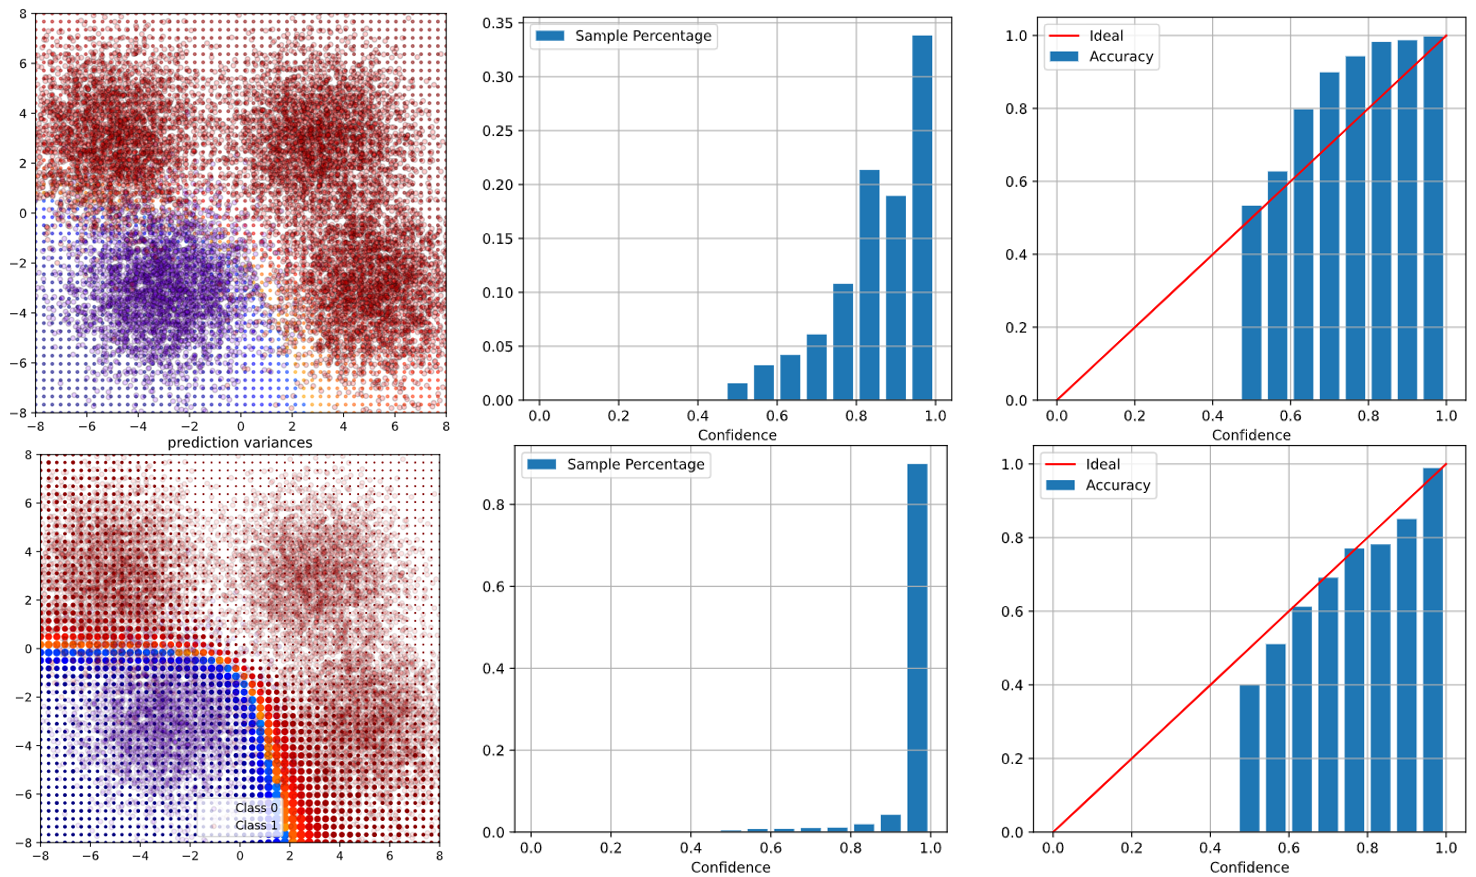
\includegraphics[width=\textwidth]{figs/2d_classification_ece_acc.png}
	\caption{Classification example for basic MLP (first row) and stochastic MLP (second row)}
	\label{fig: mlp classification}
\end{figure}

The upper left plot in Figure~\ref{fig: mlp classification} shows the data clusters and the decision boundary of a basic 2-layer MLP. 
The red clusters have some overlap with the purple cluster, and the color of the grid points indicates the classification results.
We can see the grid points near the purple cluster are assigned blue color, while the rest are assigned to red color.
The decision boundary is a curved line that roughly splits the two classes, and the classification accuracy is 95.3\%.
Meanwhile, the lower left plot shows the results from a 2-layer stochastic MLP.
A clear difference is a measurement of uncertainty, which is indicated by the size of the grid points. 
Since the stochastic model is migrated from a deterministic one, the stochastic boundary is very close to the deterministic one. 
From the plot, we observe reasonable high uncertainty near the boundary, and low uncertainty else where. 

In the plots for confidence-accuracy gap, the red line represents the ideal case, where the confidence perfectly matches the actual accuracy.
From the plots, we observe better calibration results in the stochastic model (lower right plot).
The main reason is the stochastic model correctly classified over 80\% of data points, with matching confidence. 
As a result, the deterministic MLP has an ECE at 0.094, while the stochastic model has only 0.009.

To investigate the effect of flow, we compare the training progress of stochastic MLPs with different flow lengths. 
Figure~\ref{fig: mlp with different flows} shows the trends of ELBO, likelihood and KL divergence at each training epochs.
For this example, we use planar flow, and only change the length.
As a special case, length 0 means the stochastic part has merely a learnable Gaussian distribution.
From the plots, we observe that flow length 12 results in highest likelihood and ELBO, and flow length 0 gives lowest values.
Therefore, the a flow part with reasonable length (12 here) could improve the model performance. 

\begin{figure}[H]
	\centering
	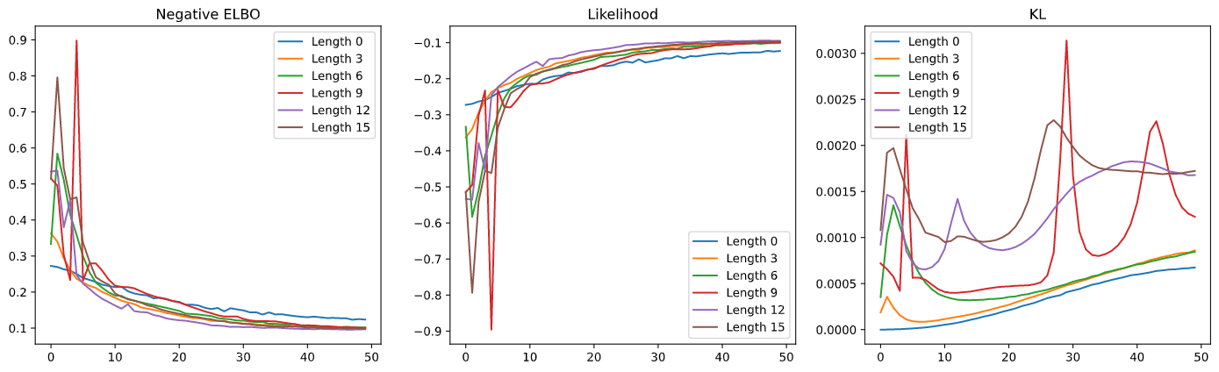
\includegraphics[width=\textwidth]{figs/2d_classification_flow_len.png}
	\caption{Training progress of stochastic MLPs with different flow lengths ($x$ axis is epoch)}
	\label{fig: mlp with different flows}
\end{figure}

\end{rSubsection}



\begin{rSubsection}{Image Classification}
In this section, we compare flow-based LeNet~\cite{lecun1998gradient} and VGG~\cite{simonyan2014very} with their deterministic baseline.
Since images are high-dimensional data, we don't have good methods to visualize the output uncertainty.
But we can still observe the training progress in Figure~\ref{fig: sto lenet} and Figure~\ref{fig: sto vgg}.

Figure~\ref{fig: sto lenet} presents the training progress of LeNet-based models on FashionMnist~\cite{xiao2017fashion} and CIFAR-10~\cite{krizhevsky2009CIFAR}. 
The three plots in the first row shows the trend of training losses, i.e., ELBO, log likelihood and KL Divergence. 
Compared to the "no flow" version, the flow based model has higher data likelihood, higher KL divergence and larger ELBO for both datasets. 
Same as before, the models labeled with "no flow" has only a learnable Gaussian distribution in the stochastic part of each layer.
Higher data likelihood means the flow-based models can better fit the data, and higher KL divergence indicates that the flow based posterior deviates farther from the prior (Gaussian here), compared to the learnable Gaussian. 

The two plots in the second row records the testing accuracy and ECE in each training epoch. 
Both the flow-based model and its "no flow" version has outperformed the deterministic baseline after a few training epochs.
Compared to the baseline, the improvements of stochastic models on CIFAR-10 is more evident than that on FashionMnist.
A possible reason is the capacity basic LeNet is enough to handle the complexity of FashionMnist (nearly 90\% baseline accuracy).
Therefore the extra capacity introduced by the flows won't have significant effects.
If we move to CIFAR-10, the effects of flows begin to manifest as the classification problem becomes more difficult.
And the flow based model has about 2\% higher accuracy than the "no flow" version. 
However, the expected calibration loss is more unpredictable.
While the baseline model is nicely calibrated, with ~1.5\% ECE on both datasets, the stochastic models could have even higher ECE.

Besides, the input augmentation in our stochastic layer has similar mechanisms to Dropout.
But the difference is, dropout applies binary random variable to the input, while our stochastic layer adopts real-valued augmentation. 
Since the basic LeNet does not have dropout layers, we also extended it with dropout and recorded the best accuracy and ECE as another baseline. 
As a result, dropout didn't improve the classification accuracy, and the ECE (up to 5\%) is also higher than the basic LeNet.

\begin{figure}[H]
	\centering
	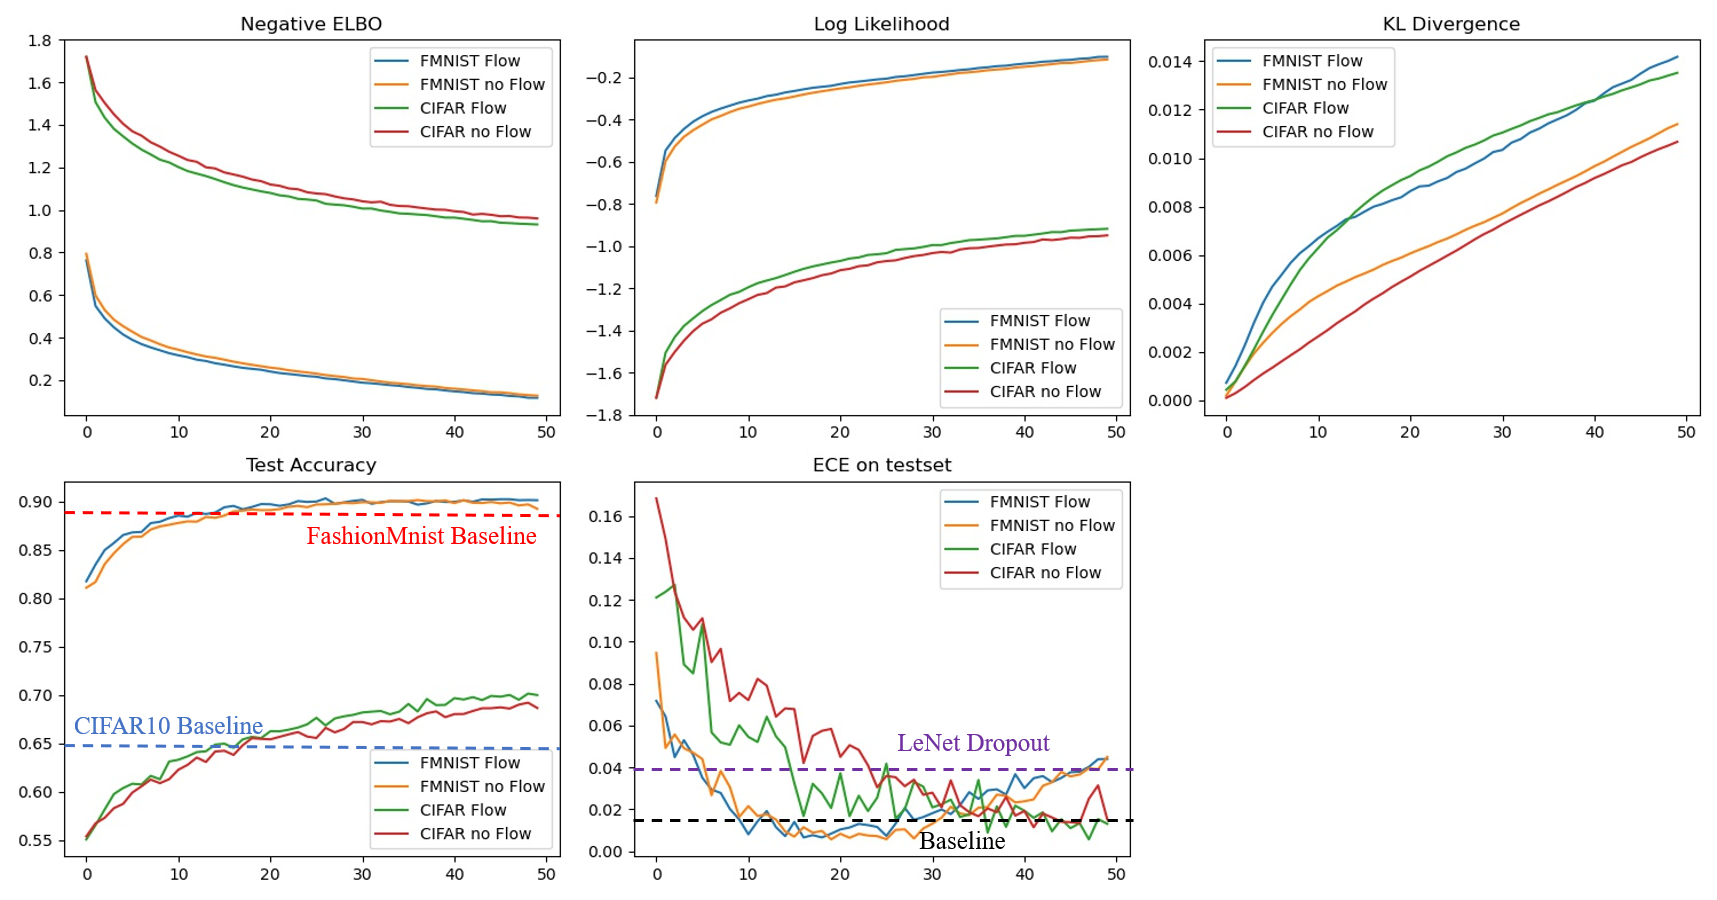
\includegraphics[width=\textwidth]{figs/stolenet results.png}
	\caption{Training progress of basic and stochastic LeNet ($x$ axis is epoch)}
	\label{fig: sto lenet}
\end{figure}

\begin{figure}[H]
	\centering
	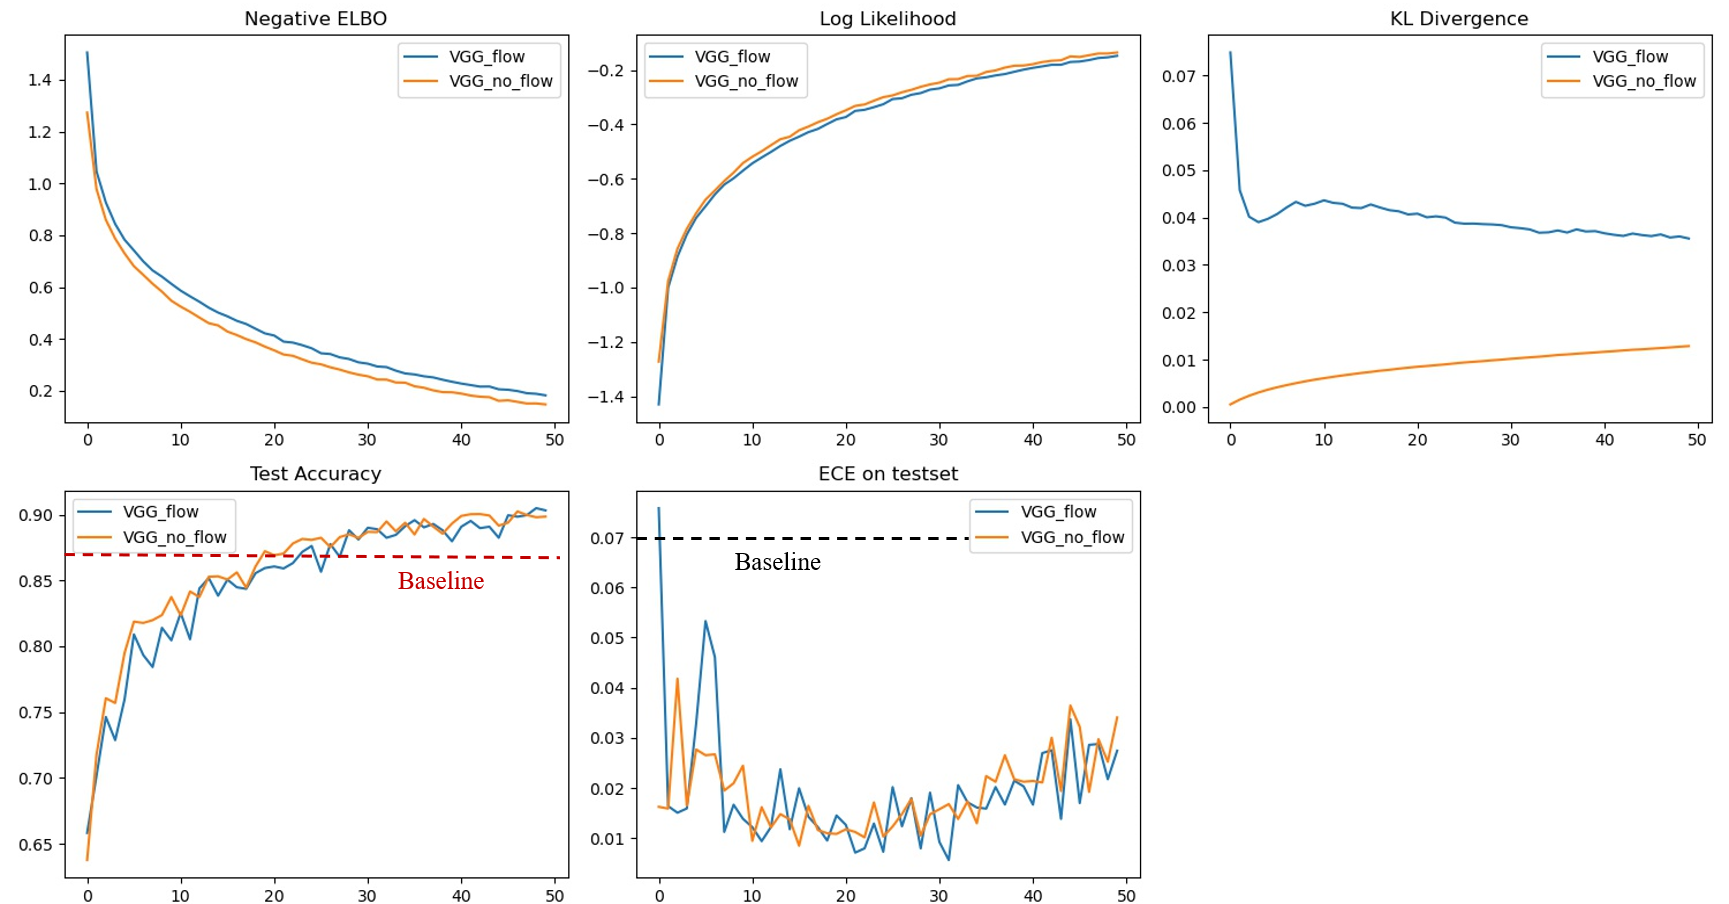
\includegraphics[width=\textwidth]{figs/stovgg results.png}
	\caption{Training progress of basic and stochastic VGG16 ($x$ axis is epoch)}
	\label{fig: sto vgg}
\end{figure}

Figure~\ref{fig: sto vgg} shows the training progress of basic and stochastic VGG16.
From the plots, we can see the flow part has almost no effect, despite the fact that both stochastic models has higher accuracies and lower ECE compared to baseline. 
Again, these experiment results are also in favour of our conjecture above.
The basic VGG16 model has enough capacity itself, because it can reach a high testing accuracy (93.15\%) on CIFAR10~\cite{sehwanjoo2020vggcifar10}.
Therefore, the flow part, which introduces extra complexity, won't have substantial effect on VGG16. 
Another evidence is the KL divergence in the flow based model, which decreases as training goes on. 
This trend means the training process is gradually leading the flow posterior back to the prior, which indicates the flow part is not necessarily helpful for higher classification accuracy.

\end{rSubsection}

\end{rSection}

\begin{rSection}{Implementation Details}

	\textbf{Flow Blocks}.

	how did you code up the flow part? what flows are used for stolenet and stovgg? 

	mention how I implemented 2d planar here.

	shall we multiply the glow log det by h*w?

	also say the number of samples for training and testing 
	
\end{rSection}

\begin{rSection}{Discussions}

	unsolved problems: lack of benchmark and metrics

	need a good way to make use of the distribution, right now we just take the mean and variance 

	how do we evaluate the quality of the posterior?

	some thoughts on possible improvements

	KL[q||p] = cross\_entropy(q, p) - entropy(q), adding an entropy to ELBO will be equivalent to multiplying "entropy(q)" by a coefficient larger than 1
	
\end{rSection}

% \begin{rSection}{The first Problem}
% 	You may briefly state how you solve this problem here
% 	\begin{rSubsection}{The first part of the problem}
% 		in the first subsection, build a list with \mintinline{latex}{\begin{rlisting}}
% 		\begin{rlisting}
% 			\item just write something random
% 			\item another random line
% 		\end{rlisting}
% 		build an ordered list with \mintinline{latex}{\begin{renum}}
% 			\begin{renum}
% 				\item just write something random
% 				\item another random line
% 			\end{renum}
% 	\end{rSubsection}

% 	\begin{rSubsection}{The second part of the problem}
% 		in the second subsection, insert a figure
% 		\begin{figure}[H]
% 			\centering
% 			\includegraphics[width=0.45\textwidth]{example-image-a}
% 			\caption{Add captions here}
% 		\end{figure}

% 		Two figures with individual numbering and caption. Comment out \mintinline{text}{\caption{}} to remove individual caption for subfigures.
% 		\begin{figure}[H]
% 			\centering
% 			\begin{subfigure}[t]{0.45\textwidth}
% 			  \centering	
% 			  \includegraphics[width=\textwidth]{example-image-a}
% 			  \caption{some comments on this figure}
% 			\end{subfigure}
% 			\qquad
% 			\begin{subfigure}[t]{0.45\textwidth}
% 			  \includegraphics[width=\textwidth]{example-image-a}
% 			  \caption{some other comments}
% 			\end{subfigure}
% 			\caption{Geometrical figures}
% 		  \end{figure}
		
% 		Text with picture left-right structure, remember to keep the blank line below (maybe not very useful)

% 		\begin{figure}[H]
% 			\begin{minipage}[b]{0.5\linewidth} % use [c] here makes the text vertically centered
% 				\centering
% 				\includegraphics[width=\textwidth]{example-image-a}
% 				\caption{some comments}
% 			\end{minipage}%
% 			\begin{minipage}[b]{0.5\linewidth} % use [c] here makes the text vertically centered
% 				\centering
% 				\begin{tabular}{|c|c|} 
% 					\hline
% 					aa & bb \\ \hline
% 					cc & dd \\ \hline
% 				\end{tabular}
% 				\captionof{table}{Table caption}
% 			\end{minipage}
% 		\end{figure}

% 		Maybe you need to cite something \cite{danelljan2014BMVC}, and you can specify the IEEE style by using in the end \mintinline{text}{\bibliographystyle{ieee_fullname}}, Elsevier Style with \mintinline{text}{elsarticle-num} and Harvard Style with \mintinline{text}{elsarticle-harv0}.
% 		After this, please compile the tex file with \mintinline{text}{pdflatex->bibtex->pdflatex->pdflatex}.
% 		If the main text has not cited anything, just use \mintinline{text}{pdflatex}
% 	\end{rSubsection}
% \end{rSection}


% Sometimes we need to start a new page with \mintinline{latex}{\newpage} for a new question.
% \newpage
% \begin{rSection}{A new section for a new problem}
% \begin{rSubsection}{the first step}
% 	this is for inserting codes with or without a bounding box, remember to use \mintinline{text}{PDFLaTeX}

% 	\begin{minted}[tabsize=4, bgcolor=bg, autogobble, escapeinside=||, frame=single]{python}
% 		import numpy as np
% 		def some_function(some_variables):
% 			pass
% 		# even put an under line in codes
% 		|\ul{undelrine}| 
% 	  \end{minted}
% 	You will need to explain the codes a bit.

% 	\begin{mdframed}[backgroundcolor=bg]
% 	\begin{minted}[tabsize=4, autogobble, escapeinside=||]{python}
% 		import numpy as np
% 		def some_function(some_variables):
% 			pass
% 	\end{minted}
% 	\end{mdframed}
% 	You will need to explain the codes a bit.
% \end{rSubsection}

% \begin{rSubsection}{the second step}
% 	We may need to type matrix equations 
% 	\begin{equation}
% 		T = 
% 		\left[\begin{matrix} m_u & 0 & 0 \\0 & m_v & 0 \\ 0 & 0 & 1 \end{matrix}\right]
% 		\left[\begin{matrix} 1 & 0 & u_{0} \\0 & 1 & v_{0} \\ 0 & 0 & 1 \end{matrix}\right]
% 		\left[\begin{matrix} f & 0 & 0 \\0 & f & 0 \\ 0 & 0 & 1 \end{matrix}\right]
% 		=
% 		\left[\begin{matrix} fm_u & 0 & u_0 \\0 & fm_v & v_0 \\ 0 & 0 & 1 \end{matrix}\right].
% 	\end{equation}
% 	If you don't want the auto numbering 
% 	$$
% 		T = \left[\begin{matrix} m_u & 0 & 0 \\0 & m_v & 0 \\ 0 & 0 & 1 \end{matrix}\right]
% 		\left[\begin{matrix} 1 & 0 & u_{0} \\0 & 1 & v_{0} \\ 0 & 0 & 1 \end{matrix}\right]
% 		\left[\begin{matrix} f & 0 & 0 \\0 & f & 0 \\ 0 & 0 & 1 \end{matrix}\right]
% 		=
% 		\left[\begin{matrix} fm_u & 0 & u_0 \\0 & fm_v & v_0 \\ 0 & 0 & 1 \end{matrix}\right].
% 	$$
% 	or build a table to present data
% 	\begin{table}[H]
% 		\centering
% 		\caption{Some random numbers}
% 		\begin{tabular}{c|cccc}
% 			\toprule
% 			($\alpha$, $u$)& 0.7 & 0.8 & 0.9 & 1 \\
% 			\midrule
% 			1 & 25.3183 & 25.5442& 25.7192& 25.8589 \\
% 			2 & 36.8104 & 37.6098 &38.2343 & 38.7359\\
% 			3 & 44.1152 & 46.6144 & 48.6152 & {50.2597} \\
% 			4 & 39.3190& 44.5661&\textcolor{red}{48.3255} &\textcolor{red}{51.3635} \\
% 			5 & 18.0562& 35.4232 &42.3844 &47.0238 \\
% 			\bottomrule
% 		\end{tabular}
% 	\end{table}
% \end{rSubsection}
% \end{rSection}

% \bibliographystyle{ieee_fullname}
\bibliographystyle{elsarticle-num}
% \bibliographystyle{elsarticle-harv}
\bibliography{EXAMPLE_BIB}

\clearpage

\end{document}
